% Convert with command:
% convert -density 300 pic.pdf -quality 90 pic.png
\documentclass[crop,tikz,border=0pt]{standalone}
\usetikzlibrary{arrows.meta, fit}
\begin{document}

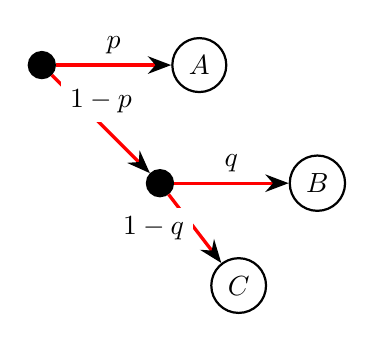
\begin{tikzpicture}
\begin{scope}[every node/.style={circle,thick,draw}]
    \node (start) at (0, 0) [shape=circle, fill=black] {};
    \node (A) at (2, 0) [shape=circle,draw=black,fill=white] {$A$};

    \node (mid) at (1.5, -1.5) [shape=circle,draw=black,fill=black] {};

    \node (B) at (3.5, -1.5) [shape=circle,draw=black,fill=white] {$B$};

    \node (C) at (2.5, -2.8) [shape=circle,draw=black,fill=white] {$C$};
\end{scope}

\begin{scope}[>={Stealth[black]},
              every node/.style={fill=white,rectangle,above},
              every edge/.style={draw=red,very thick}]
    \path [->] (start) edge node {$p$} (A);
    \path [->] (start) edge node {$1 - p$} (mid);
    \path [->] (mid) edge node {$q$} (B);
    \path [->] (mid) edge node[anchor=mid east] {$1 - q$} (C);
\end{scope}
\end{tikzpicture}

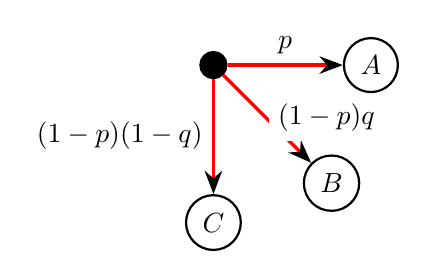
\begin{tikzpicture}
\begin{scope}[every node/.style={circle,thick,draw}]
    \node (start) at (0, 0) [shape=circle, fill=black] {};
    \node (A) at (2, 0) [shape=circle,draw=black,fill=white] {$A$};

    \node (B) at (1.5, -1.5) [shape=circle,draw=black,fill=white] {$B$};

    \node (C) at (0, -2) [shape=circle,draw=black,fill=white] {$C$};
\end{scope}

\begin{scope}[>={Stealth[black]},
              every node/.style={fill=white,rectangle,above},
              every edge/.style={draw=red,very thick}]
    \path [->] (start) edge node {$p$} (A);
    \path [->] (start) edge node [anchor=mid west] {$(1 - p)q$} (B);
    \path [->] (start) edge node [anchor=mid east] {$(1 - p)(1 - q)$} (C);
\end{scope}
\end{tikzpicture}


\end{document}
